\documentclass[12pt]{article}

%%%%%%%%%%%%%%%%%%%%%%%% PREAMBLE %%%%%%%%%%%%%%%%%%%%%%%%

% Global margins for the document:
\usepackage[
    top=0.6cm,
    left=0.6cm,
    bottom=2cm,
    right=0.6cm,
]{geometry}

% Define spacing between paragraphs in the document:
\setlength{\parindent}{0.5cm} % default indentation before the first line of a paragraph.
\setlength{\topskip}{0.2cm} % indentation at the begging of the first paragraph of every page:
\setlength{\parskip}{0.3cm} % indentation after every paragraph

% Font configurations:
\usepackage{fontspec}
\setmainfont{FreeSerif}

% For justify and some other alignment extensions:
\usepackage{ragged2e}

% Math related packages:
\usepackage{amsmath, amssymb, amsthm}
% For vectors:
\usepackage{esvect}
% Proper calculates where the not line should be drawn:
\usepackage{centernot}
% Theorem definitions:
\newtheorem{thm}{Theorem}
\newtheorem{lem}[thm]{Lemma} % a lemma that shares a counter with the Theorem.
\newtheorem{defn}{Definition}
% Package for systems:
\usepackage{systeme}
% For graphs:
\usepackage{tikz}
\usepackage{pgfplots}

% Embedding *.jpg abd *.png images
\usepackage{graphicx}
\graphicspath{{data/}{../data/}} % define the path to the images

% Provides an underline command which will break over line ends:
\usepackage{ulem}

% Better lines for tables:
\usepackage{hhline}

% Allows enumerate environment to customize the label:
\usepackage{enumitem}

% Multirow :
\usepackage{multirow}

% To use arrays:
\usepackage{array}

% Custom commands for table alignment when dealing with a lot of text (needs array and ragged2e):
\newcolumntype{L}[1]{>{\raggedright\let\newline\\\arraybackslash\hspace{0pt}}m{#1}}
\newcolumntype{C}[1]{>{\centering\let\newline\\\arraybackslash\hspace{0pt}}m{#1}}
\newcolumntype{R}[1]{>{\raggedleft\let\newline\\\arraybackslash\hspace{0pt}}m{#1}}

% Hyper links to places inside the document:
\usepackage{hyperref}
\hypersetup{
    colorlinks=true,
    % These take rgb values as a fraction of n/255.
    % That is really not how RGB works!
    linkcolor=[rgb]{0.1, 0.2, 1},
    filecolor=[rgb]{0.1, 0.2, 1},
    urlcolor=[rgb]{0.1, 0.2, 1},
    citecolor=[rgb]{0.1, 0.2, 1},
    unicode=true,
}
\urlstyle{same}

% For fancy programming code formatting and coloring:
\usepackage{minted}

% For pretty quotes:
\usepackage{epigraph}
\setlength\epigraphwidth{1\textwidth}
\setlength\epigraphrule{0pt}

% For a footer and header:
\usepackage{fancyhdr}
\pagestyle{fancy}

% \fancyhead[L]{Top Left Head}
% \fancyhead[C]{Center Head}
% \fancyhead[R]{Top Right Head}

% \fancyfoot[L]{Bottom Left Foot}
\fancyfoot[C]{Page \thepage}
% \fancyfoot[R]{Bottom Right Foot}

% Bibliography:
\usepackage{csquotes}
\usepackage[backend=biber]{biblatex}
\addbibresource{init.bib}

% For inserting loremipsum random text:
\usepackage[pangram]{blindtext}

% Allows adding sub tex files to the main tex file:
\usepackage{subfiles} % Best loaded last in the preamble

%%%%%%%%%%%%%%%%%%%%%%%% DOCUMENT STARTS HERE %%%%%%%%%%%%%%%%%%%%%%%%
\begin{document}

\begin{titlepage}
    \begin{center}
        \huge
        \textbf{Решения на задачи по \\ Линейна Алгебра}

        \large \vfill
        Последна промяна на \today
    \end{center}
\end{titlepage}
\newpage

% TOC:
\tableofcontents
\newpage

\section{Линейни Системи}

\subsection{Метода на Гаус}

\noindent Решаване на системи уравнения по Метода на Гаус, още познато като линейна елиминация.

\noindent Една линейна система запазва еднакво множеството от решения при трансформация чрез една от тези операции:
\begin{enumerate}
    \item Един ред от системата може да се размени с друг.
    \item Едно от уравненията може да се умножи по ненулева константа.
    \item Уравнение на един ред, умножено с число, може да се прибави към уравнение на друг ред.
\end{enumerate}

\noindent Тези операции се правят докато:
\begin{enumerate}
    \item Се намери непротиворечива стойността на една от търсените променливи. \textbf{Тогава имаме решение.}
    \item Се стигне до логическо противоречие, например $0=-1$. \textbf{Тогава нямаме решение.}
    \item Се останови, че нито една от стъпките не води до опростяване на кякой от редовете. \textbf{Тогава имаме безкрайно много решения.}
\end{enumerate}

\subfile{sections/gauss_method_examples.tex}
\subfile{sections/ex_1.17.tex}
\subfile{sections/ex_1.18.tex}
\subfile{sections/ex_1.19.tex}
\subfile{sections/ex_1.20.tex}
\subfile{sections/ex_1.21.tex}
\subfile{sections/ex_1.22.tex}
\subfile{sections/ex_1.23.tex}

\subsection{Намиране на множеството от решения}

\subfile{sections/describing_the_solution_set_example.tex}
\subfile{sections/ex_2.15-17.tex}
\subfile{sections/ex_2.18.tex}
\subfile{sections/ex_2.19.tex}

\subsection{Общото решение = Специфичното решение + хомогенното решение}

\noindent Всяка линейна система, която е в ешелонна форма, има множество от решения в следната форма:
\begin{equation*}
    \{ \vv{p} + c_{1}\vv{\beta}_{1} + \cdots + c_{k}\vv{\beta}_{k}\ |\ c_{1},...,c_{k} \in \mathbb{R}\}
\end{equation*}

\noindent Където вектора $\vv{p}$ е специфично решение и броя на векторите $\vv{\beta}_{1} ... \vv{\beta}_{k}$ е равен на броя \textbf{свободни променливи}.

\noindent Линейните уравнения са \textbf{хомогенни} ако имат константа равна на 0, а една система е \textbf{хомогенна} когато всички уравнения са \textbf{хомогенни}:
\begin{equation*}
    a_{1}x_{1} + a_{2}x_{2} + \cdots + a_{n}x_{n} = 0
\end{equation*}

\noindent Когато системата е хомогенна тя няма специфично решение $\vv{p} = 0$, а множеството от решения има следната форма:
\begin{equation*}
    \{ c_{1}\vv{\beta}_{1} + \cdots + c_{k}\vv{\beta}_{k}\ |\ c_{1},...,c_{k} \in \mathbb{R}\}
\end{equation*}

\noindent Друго характерно за хомогенните системи е, че те винаги имат едно уникално решение или безброй много решения.

\subfile{sections/ex_3.14.tex}
\subfile{sections/ex_3.15.tex}

\section{Линейна Геометрия}

Трите видя решения (които разгеждахме в предишната глава) на една система от линейни уравнения могат да се представят геометрично:

\noindent \hspace{5pt} Unique Solution \hspace{0.2\linewidth} No Solution \hspace{0.2\linewidth} Infnitely many solutions \hspace{0.2\linewidth}{3em}

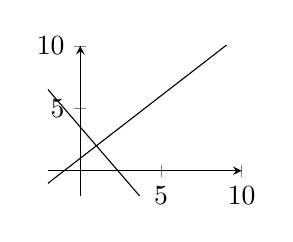
\begin{tikzpicture}
    \begin{axis}[xmin=-2,
        xmax=10,
        ymin=-2,
        ymax=10,
        axis x line=middle,
        axis y line=middle,
        samples=20,
        width=0.33333333\textwidth]

        \addplot[domain=-20:20]{(7 - 3*x) / 2};
        \addplot[domain=-20:20]{x + 1};
    \end{axis}
\end{tikzpicture}
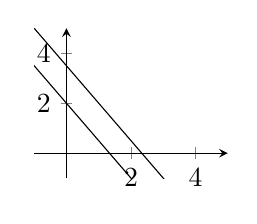
\begin{tikzpicture}
    \begin{axis}[xmin=-1,
        xmax=5,
        ymin=-1,
        ymax=5,
        axis x line=middle,
        axis y line=middle,
        samples=20,
        width=0.33333333\textwidth]

        \addplot[domain=-20:20]{(7 - 3*x)/2};
        \addplot[domain=-20:20]{(4 - 3*x)/2};
    \end{axis}
\end{tikzpicture}
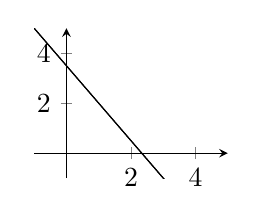
\begin{tikzpicture}
    \begin{axis}[xmin=-1,
        xmax=5,
        ymin=-1,
        ymax=5,
        axis x line=middle,
        axis y line=middle,
        samples=20,
        width=0.33333333\textwidth]

        \addplot[domain=-20:20]{(7 - 3*x)/2};
        \addplot[domain=-20:20]{(14 - 6*x)/4};
    \end{axis}
\end{tikzpicture}

\hspace{2pt}
\noindent $ \sysdelim..\systeme{
    3x + 2y = 7,
    x - y = -1
}$ \hspace{0.2\linewidth} $ \sysdelim..\systeme{
    3x + 2y = 7,
    3x + 2y = 4
}
$ \hspace{0.2\linewidth} $ \sysdelim..\systeme{
    3x + 2y = 7,
    6x + 4y = 14
}
$

\subsection {Вектори}

\noindent Векторите са обекти с посока и величина/магнитут. Два вектора с еднаква посока и еднакъв магнитут са еднакви, \textbf{дори когато имат различна начална точка}.

\noindent Можем да опишем вектор $ (x_{1}, y_{1}) $ до $ (x_{2}, y_{2}) $ по следния начин:

\begin{equation*}
    \left(\begin{array}{ c }x_{1} - x_{2} \\ y_{1} - y_{2} \end{array}\right)
\end{equation*}

\noindent или по-генерализирано:

\begin{equation*}
    \overrightarrow{v} = \left(\begin{array}{ c }v_{1} \\ v_{2} \end{array}\right)
\end{equation*}

\noindent където $ \overrightarrow{v} $ започва в някоя избрана начална точка и приключва на $ (v_{1}, v_{2}) $ разтояние от тази точка.

\noindent Можем да дефинираме множеството от реалните числа по следния начин (тук \textbf{нарочно} не правим голяма разлика между вектор и точка):

\begin{equation*}
    \mathbb{R}^{n} = \{ \left(\begin{array}{ c }v_{1} \\ \vdots \\ v_{n} \end{array}\right) \mid v_{1},\ \ldots\ , v_{n} \in \mathbb{R} \}
\end{equation*}

\subsection{Линия}

\noindent Линия в $ \mathbb{R}^2 $ от $ (1, 2) $ до $ (3, 1) $ може да се представя с два вектора в следното множеството:

\begin{equation*}
    \{ \left(\begin{array}{ c } 1 \\ 2 \end{array}\right) + t \left(\begin{array}{ c } 3 - 1 \\ 1 - 2 \end{array}\right) \mid t \in \mathbb{R} \}
\end{equation*}

\noindent след сметките:

\begin{equation*}
    \{ \left(\begin{array}{ c } 1 \\ 2 \end{array}\right) + t \left(\begin{array}{ c } 2 \\ -1 \end{array}\right) \mid t \in \mathbb{R} \}
\end{equation*}

\subsection{Равнина (plain)}

\noindent Равнина в $ \mathbb{R}^3 $ през точките $(1,0,5)$, $(2,1,-3)$ и $(-2, 4, 0.5)$ може се представи с три вектора в множеството:

\begin{equation*}
    \{ \left(\begin{array}{ c } 1 \\ 0 \\ 5 \end{array}\right) + t \left(\begin{array}{ c } 2 - 1 \\ 1 - 0 \\ -3 - 5 \end{array}\right) + s \left(\begin{array}{ c } -2 - 1 \\ 4 - 0 \\ 0.5 - 5 \end{array}\right) \mid t, s \in \mathbb{R} \}
\end{equation*}

\noindent след сметките:

\begin{equation*}
    \{ \left(\begin{array}{ c } 1 \\ 0 \\ 5 \end{array}\right) + t \left(\begin{array}{ c } 1 \\ 1 \\ -8 \end{array}\right) + s \left(\begin{array}{ c } -3 \\ 4 \\ -4.5 \end{array}\right) \mid t, s \in \mathbb{R} \}
\end{equation*}

\noindent \textbf{Генерелазираната дефиниция:}

\noindent Множество в слдната форма $ \{ \vv{p} + t_{1}\vv{v}_{1} + t_{2}\vv{v}_{2} + \ldots t_{k}\vv{v}_{k} \mid t_{1},\ \ldots\ , t_{k} \}$ където $ v_{1},\ \ldots\ , v_{k} \in \mathbb{R}^n $ и $ k \leq n $, то това е k-мерна линейна повърхност (k-dimentional linear serfice) или k-flat (няма превод тва).

\textbf{
    TODO: Продължи с решаване на задачите сапочващи на 41-ва страница.
}

\end{document}